\problemname{The Bat}

The bat Båtman lives in a large cave with many other bats.
Båtman has just gotten a new job as the official bat mailman.
This means that Båtman must deliver letters between certain points in the cave.

The cave is two-dimensional and rectangular with height $H$ and width $W$ cm.
It is also filled with a total of $N$ \emph{stalagmites} and
\emph{stalactites}. A \emph{stalagmite} is a vertical dripstone formation that
grows up from the cave floor, and a \emph{stalactite} is a vertical
dripstone formation that grows down from the cave ceiling.
Both the stalagmites and the stalactites in the cave are infinitely thin, but cannot
be flown through.

Båtman has received a list of $Q$ letters that must be delivered.
Each letter must be picked up from one point in the cave and delivered to another
point. Båtman now wonders, for each letter, how far he must fly
to deliver it from the starting point to the endpoint, and asks you for
help to compute this.

Bats (including Båtman) can only fly straight up, straight down,
straight left, and straight right, but can switch between these four directions
at any time.\footnote{The reader may recognize that we are interested in \emph{Manhattan} distance in this problem.}
For example, Båtman can fly $0.4$ cm to the right, and then switch to flying
$4.3$ cm upward.

\begin{figure}[!h]
\begin{center}
  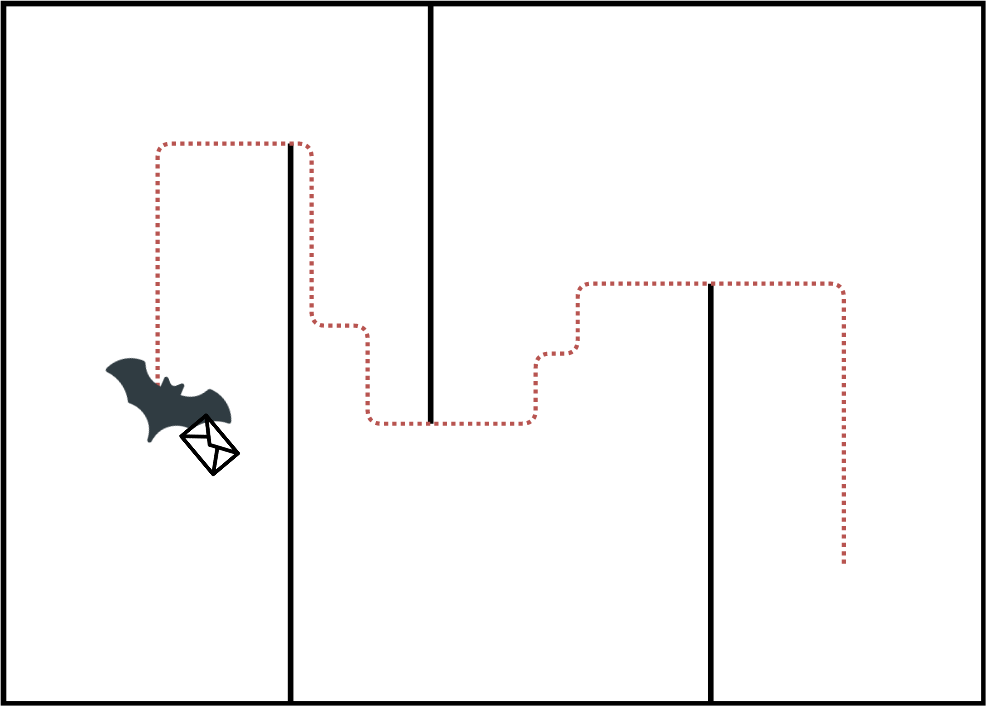
\includegraphics[width=12cm]{fladdermus.png}
\end{center}
  \caption{Illustration of the first sample. The dotted line shows
  a possible shortest flight path of length 12 for delivering the first letter.}
\end{figure}

\section*{Input}
The first line contains the four integers $N,Q,H,W$ ($1 \leq N, Q \leq 2 \cdot 10^5$, $1 \leq H,W \leq 10^9$).
Then follow $N$ lines in one of the following forms:
\begin{itemize}
  \item $1\enspace x\enspace y$, meaning that there is a stalagmite
    growing up from the point $(x,0)$ to the point $(x,y)$.
  \item $2\enspace x\enspace y$, meaning that there is a stalactite
    growing down from the point $(x,H)$ to the point $(x,y)$.
\end{itemize}
No stalagmite/stalactite reaches all the way from the ceiling to the floor,
and the stalagmites/stalactites are all entirely inside the cave,
i.e.\ $1\le x_{i} < W$ and $1\le y_{i} < H$.

Then follow $Q$ lines with four integers
$x_{1},y_{1},x_{2},y_{2}$ ($1\le x_{1},x_{2} < W$, $1\le y_{1},y_{2}< H$) representing that a letter should be delivered from
the point $(x_{1},y_{1})$ to the point $(x_{2},y_{2})$.

\textbf{It is guaranteed that all $x$-coordinates in the input are unique.}

\section*{Output}
Your program should print $Q$ lines, one for each letter.
The $i$-th line should contain an integer that is the minimum
distance Båtman must fly to deliver the $i$-th letter.

\section*{Scoring}
Your solution will be tested on a set of test groups.
To earn points for a group, you must pass all test cases in that group.

\noindent
\begin{tabular}{| l | l | l |}
\hline
\textbf{Group} & \textbf{Points} & \textbf{Constraints} \\ \hline
$1$    & $15$         & $N,Q\le 100$ and $H,W\le 500$ \\ \hline
$2$    & $20$         & $N,Q \le 2000$ and $H,W\le 2\cdot 10^6$\\ \hline
$3$    & $25$         & There are at most 15 stalactites \\ \hline
$4$    & $40$         & No additional constraints. \\ \hline
\end{tabular}
